\chapter{De la mecánica de partículas a los campos clásicos}

\section{Qué es un campo}

En la clase anterior desarrollamos la mecánica relativista de partículas a partir de una acción invariante. Ahora cambiamos el objeto dinámico. El tema es la teoría clásica de campos, no la teoría cuántica de campos. En ocasiones, la mecánica cuántica nos servirá de comparación, pero las ecuaciones de este capítulo describen campos clásicos ordinarios. El electromagnetismo es el modelo conocido que tenemos en mente: las ondas electromagnéticas se propagan por el espacio e interactúan con partículas cargadas. Comenzaremos con un campo aún más sencillo.

El espacio-tiempo puede tener muchas coordenadas espaciales, pero tiene una sola coordenada temporal. Escribimos
\begin{equation}
x^\mu=(t,x^1,\ldots,x^d),
\end{equation}
donde el índice espacial \(i=1,\ldots,d\). El número \(d\) puede ser 3, como en nuestro mundo, o 1, 2, 9, 25 o cualquier otro que resulte útil en un modelo. La asimetría importante en esta etapa es que sigue habiendo una sola dirección temporal. La clase no intenta explicar por qué las teorías con varios tiempos son tan difíciles; simplemente adopta el marco de un solo tiempo en el que se formula la física causal ordinaria.

Un campo es una magnitud medible cuyo valor puede variar de un punto a otro y con el tiempo. La temperatura es un ejemplo sencillo:
\begin{equation}
T=T(\mathbf{x},t).
\end{equation}
Asigna un número a cada suceso, por lo que es un campo escalar. La velocidad del viento también varía en el espacio y en el tiempo, pero tiene módulo y dirección y, por tanto, varias componentes; es un campo vectorial. En física relativista, los vectores naturales tienen 4 componentes en vez de 3.

Durante la mayor parte de esta clase, el campo tiene una sola componente y se denota con la letra griega correspondiente a \(f\):
\begin{equation}
\phi=\phi(\mathbf{x},t).
\label{eq:sr4-field-definition}
\end{equation}
Más adelante, llamar escalar a \(\phi\) significará algo más que decir que tiene una sola componente. Significará que todos los observadores inerciales asignan el mismo valor a \(\phi\) en un mismo suceso físico. Esa ley de transformación se introduce una vez desarrollada la mecánica variacional.

\section{El modelo de la partícula}

\subsection{Una coordenada llamada \texorpdfstring{\(\phi\)}{phi}}

La vía más rápida hacia la teoría de campos comienza por volver a una partícula no relativista ordinaria. Supongamos que la partícula se mueve sobre una recta, pero llamemos \(\phi\) a su coordenada en vez de \(x\). No hay ninguna obligación matemática de llamar \(x\) a una coordenada; elegimos ese nombre poco habitual para hacer visible la analogía que viene. Representemos el tiempo en el eje horizontal. Entonces, toda la historia de la partícula es una curva \(\phi(t)\), que puede tomar valores positivos y negativos.

Para tiempos inicial y final fijos \(a\) y \(b\), la acción es
\begin{align}
A[\phi]
&=\int_a^b dt\,L(\phi,\dot\phi),\\
L(\phi,\dot\phi)
&=\frac{m}{2}\dot\phi^{\,2}-V(\phi).
\label{eq:sr4-particle-lagrangian}
\end{align}
La ecuación de Euler--Lagrange es
\begin{equation}
\frac{d}{dt}\left(\frac{\partial L}{\partial\dot\phi}\right)
-\frac{\partial L}{\partial\phi}=0.
\label{eq:sr4-particle-el}
\end{equation}
Para el lagrangiano de \eqref{eq:sr4-particle-lagrangian},
\begin{equation}
\frac{\partial L}{\partial\dot\phi}=m\dot\phi,
\qquad
\frac{\partial L}{\partial\phi}=-\frac{dV}{d\phi},
\end{equation}
de modo que
\begin{equation}
\boxed{m\ddot\phi=-\frac{dV}{d\phi}}.
\label{eq:sr4-newton}
\end{equation}
Esta es simplemente la ecuación de Newton, escrita tomando \(\phi\) como coordenada.

\begin{figure}[htbp]
\centering
\includegraphics[width=0.90\textwidth]{lecture_04_figure_01.png}
\caption{La ecuación ordinaria de Euler--Lagrange y su resultado newtoniano para la coordenada \(\phi(t)\).}
\lectureframe{00:10:18}
\end{figure}

La trayectoria física hace estacionaria la acción mientras se mantienen fijos los extremos. A menudo, en la clase se dice \emph{mínimo}, pero el enunciado preciso es que la acción es estacionaria: la trayectoria puede corresponder a un mínimo, un máximo u otro valor estacionario. Un modelo mental útil consiste en dividir el intervalo temporal en muchos tramos pequeños. La acción se convierte entonces en una función de los numerosos valores de \(\phi\) muestreados. Desplazar esos valores, manteniendo fijos los extremos, y derivar con respecto a cada uno de ellos es el antecedente en dimensión finita de la ecuación de Euler--Lagrange.

\subsection{La mecánica como teoría en dimensiones \texorpdfstring{\(0+1\)}{0+1} }

Imaginemos ahora un mundo con tiempo, pero sin dimensiones espaciales. Su espacio consta de un solo punto. Un campo en ese mundo no puede depender de la posición, porque no hay ninguna posición de la que pueda depender; solo puede ser una función \(\phi(t)\). Por tanto, la mecánica ordinaria de una coordenada puede interpretarse como una teoría de campos en dimensiones \(0+1\). Las matemáticas no han cambiado. Solo ha cambiado la interpretación: de la posición de una partícula al valor de un campo en un mundo sin espacio.

\begin{figure}[htbp]
\centering
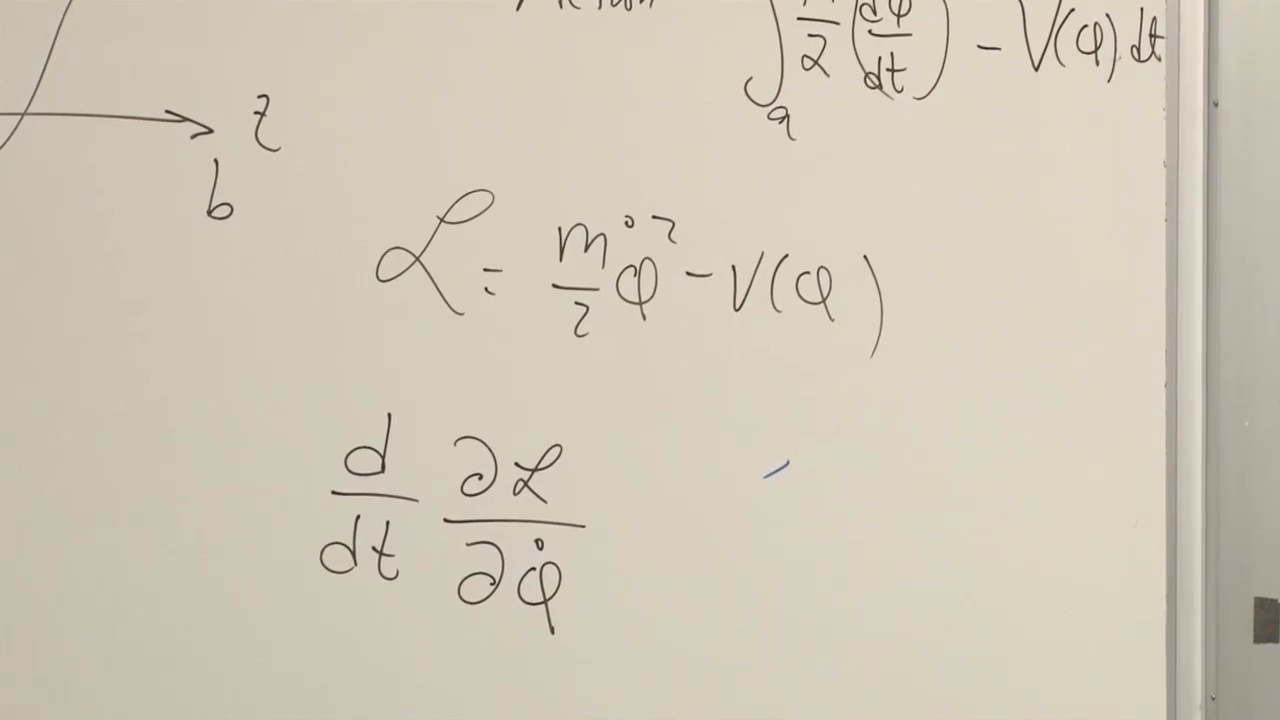
\includegraphics[width=0.90\textwidth]{lecture_04_figure_02.png}
\caption{La historia muestreada \(\phi(t)\): una trayectoria de partícula y, con una nueva interpretación, una historia de campo en dimensiones \(0+1\).}
\lectureframe{00:14:30}
\end{figure}

\begin{classroomqa}
\audiencequestion{¿Desaparece el potencial si no hay dimensiones espaciales?}
\lecturerresponse{No. Desaparece la variación espacial, pero el campo sigue teniendo un valor. La energía puede depender de ese valor mediante \(V(\phi)\). En la interpretación de partícula, desplazar la curva hacia arriba o hacia abajo cambia la energía potencial; en la interpretación de campo, distintos valores de \(\phi\) conllevan distintas energías potenciales. \lecturetimestamp{00:15:00}}
\end{classroomqa}

\begin{classroomqa}
\audiencequestion{En vez de imaginar que no hay espacio en absoluto, ¿se puede imaginar un espacio ordinario en el que el campo dependa solo del tiempo?}
\lecturerresponse{Sí. Para este propósito, las matemáticas locales son las mismas: todas las derivadas espaciales se anulan y solo queda \(\phi(t)\). Llamarla teoría en dimensiones \(0+1\) permite aislar esa estructura reducida, pero un campo espacialmente homogéneo en un mundo de mayor dimensión ofrece la misma intuición. \lecturetimestamp{00:16:25}}
\end{classroomqa}

Ahora queda claro el propósito de este rodeo. Conocemos el principio de acción para un campo que depende de una sola coordenada: el tiempo. Podemos utilizar ese patrón para conjeturar el principio de acción de un campo que depende de todas las coordenadas del espacio-tiempo.

\section{Una historia de campo sobre el espacio-tiempo}

\subsection{De una curva a una superficie}

En dimensiones \(1+1\), el espacio-tiempo es un plano con coordenadas \(t\) y \(x\). El valor \(\phi(x,t)\) aporta una tercera dirección. Por tanto, la historia del campo no es una curva, sino una superficie sobre el plano del espacio-tiempo. La superficie puede elevarse por encima de cero o descender por debajo de cero, porque un campo escalar no tiene por qué ser positivo.

\begin{figure}[htbp]
\centering
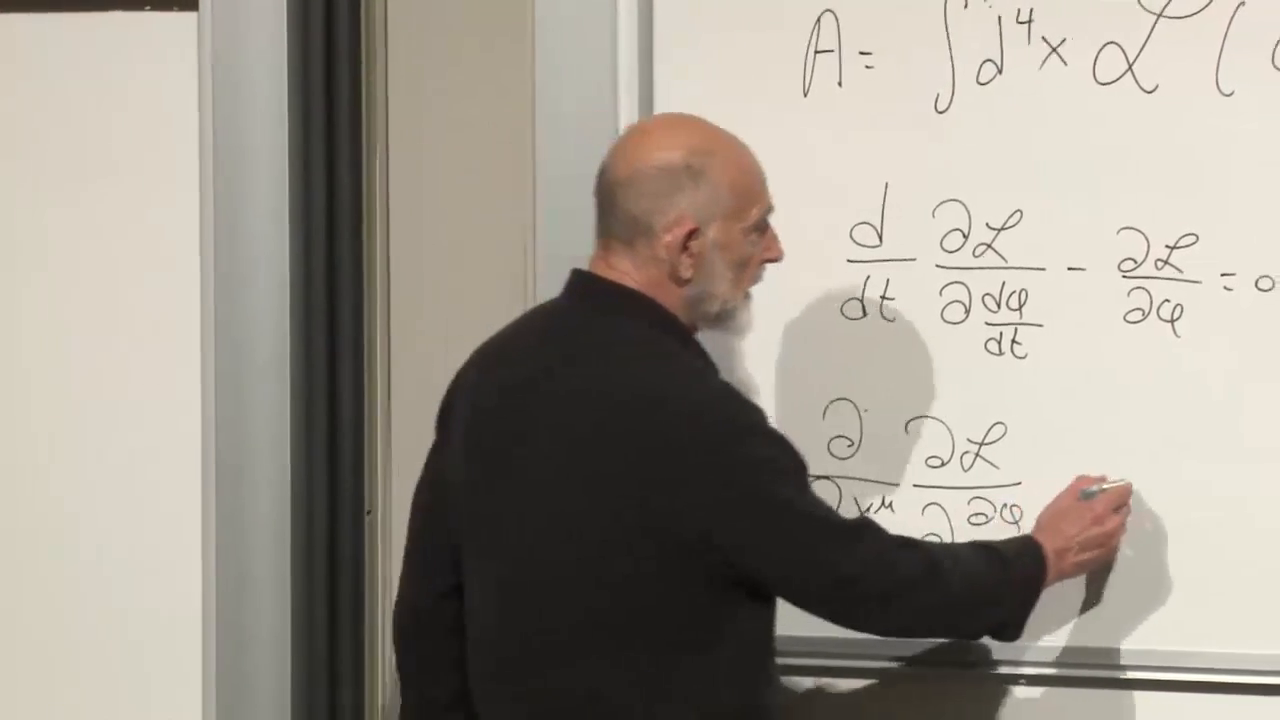
\includegraphics[width=0.90\textwidth]{lecture_04_figure_03.png}
\caption{La historia de un campo escalar representada como una superficie sobre un plano de espacio-tiempo de dimensiones \(1+1\).}
\lectureframe{00:20:46}
\end{figure}

Nuestro espacio-tiempo físico se denomina de dimensiones \(3+1\): 3 dimensiones de espacio y 1 de tiempo. Un modelo sobre una mesa tiene dimensiones \(2+1\), y unas cuentas restringidas a un alambre sugieren un mundo de dimensiones \(1+1\). El eje adicional necesario para representar \(\phi\) hace imposible incluso dibujar fielmente el caso \(3+1\), pero la definición no presenta ambigüedad: una historia completa asigna un valor de \(\phi\) a cada suceso del espacio-tiempo.

\subsection{De extremos fijos a datos de contorno fijos}

El problema variacional de la partícula fija dos extremos y varía la curva entre ellos. El análogo en teoría de campos selecciona una región del espacio-tiempo, fija \(\phi\) en el contorno de esa región y varía \(\phi\) en su interior. La región puede ser un rectángulo en un dibujo de dimensiones \(1+1\), o cualquier región adecuada en un espacio-tiempo de mayor dimensión.

\begin{figure}[htbp]
\centering
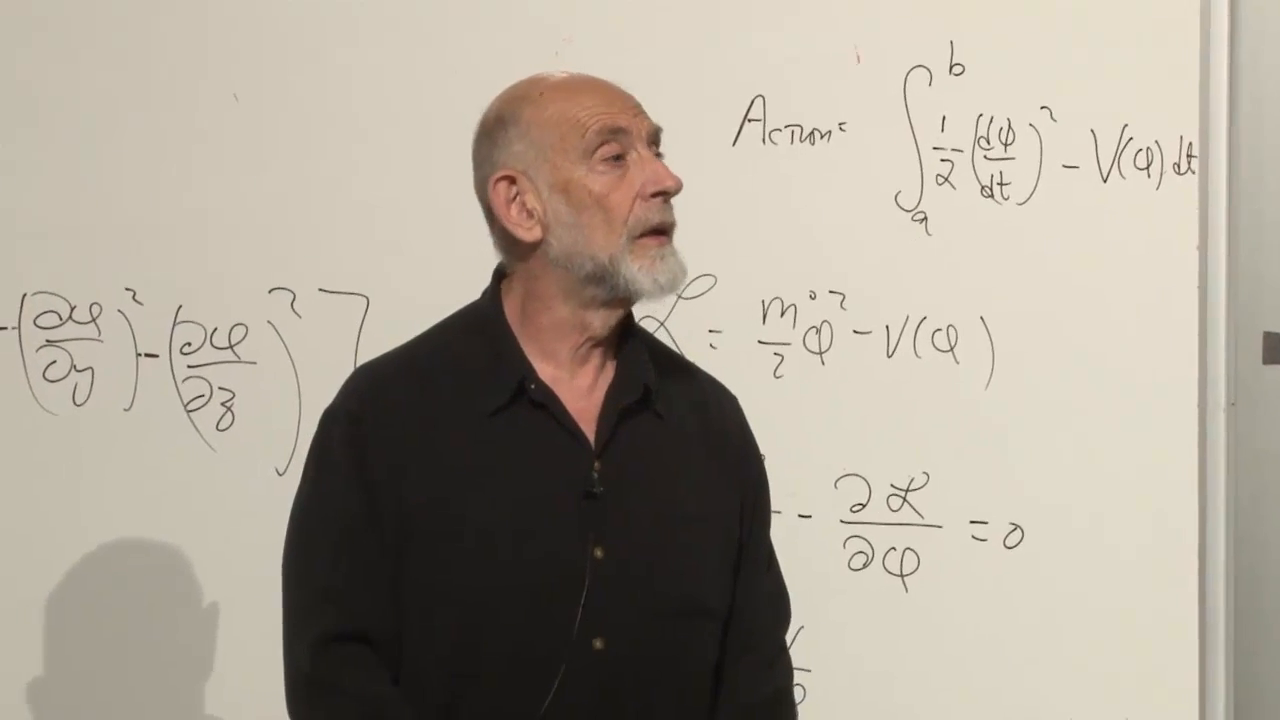
\includegraphics[width=0.90\textwidth]{lecture_04_figure_04.png}
\caption{Una región del espacio-tiempo cuyo contorno completo se mantiene fijo mientras se varía el campo en el interior.}
\lectureframe{00:24:52}
\end{figure}

\begin{classroomqa}
\audiencequestion{¿Sigue funcionando la formulación lagrangiana cuando el potencial depende explícitamente del tiempo?}
\lecturerresponse{Sí. Las formulaciones de Euler--Lagrange y hamiltoniana siguen funcionando. En general, lo que se pierde es la conservación de la energía: la dependencia explícita del tiempo rompe la simetría de traslación temporal. En teoría de campos, el enunciado correspondiente es que se permite la dependencia explícita del espacio-tiempo, aunque afecta a las leyes de conservación asociadas. \lecturetimestamp{00:23:49}}
\end{classroomqa}

\begin{classroomqa}
\audiencequestion{Para la región rectangular del campo, ¿se fijan solo los lados superior e inferior o todo el contorno?}
\lecturerresponse{En esta construcción variacional se fija todo el contorno: los 4 lados del rectángulo de dimensiones \(1+1\). El campo solo puede fluctuar en el interior. Este es el análogo directo de mantener fijos ambos extremos en la mecánica de partículas. \lecturetimestamp{00:24:24}}
\end{classroomqa}

Fijar todo el contorno es una condición sobre la variación que se utiliza para derivar las ecuaciones. Cuando se trata la ecuación de campo hiperbólica resultante como un problema de evolución física, es más habitual especificar datos iniciales adecuados y dejar que la ecuación los propague hacia adelante en el tiempo.

\section{La acción y la ecuación de Euler--Lagrange del campo}

\subsection{La densidad lagrangiana}

Dividamos la región del espacio-tiempo en celdas pequeñas. Se supone que la acción es una suma de contribuciones locales, una por cada celda. En el límite continuo, esa suma se convierte en una integral sobre el espacio-tiempo:
\begin{equation}
A[\phi]
=
\int_{\Omega} d^4x\,
\mathcal{L}\!\left(
\phi,\partial_\mu\phi;x^\mu
\right),
\qquad
d^4x=dt\,dx\,dy\,dz.
\label{eq:sr4-field-action}
\end{equation}
La magnitud \(\mathcal{L}\) es la densidad lagrangiana. El punto y coma en \(\mathcal{L}(\phi,\partial_\mu\phi;x^\mu)\) separa los argumentos dinámicos de la posible dependencia explícita de las coordenadas. En un sistema cerrado y homogéneo, esta última dependencia suele estar ausente, pero el formalismo variacional no la prohíbe.

La notación compacta
\begin{equation}
\partial_\mu\phi
\equiv
\frac{\partial\phi}{\partial x^\mu}
\end{equation}
agrupa las derivadas temporales y espaciales. En la notación por componentes de la clase, también se puede escribir
\begin{equation}
\begin{aligned}
\phi_t&=\frac{\partial\phi}{\partial t},\\
\phi_x&=\frac{\partial\phi}{\partial x},\\
\phi_y&=\frac{\partial\phi}{\partial y},\\
\phi_z&=\frac{\partial\phi}{\partial z}.
\end{aligned}
\label{eq:sr4-component-derivatives}
\end{equation}
Puede haber varios campos, igual que una partícula puede tener varias coordenadas. Por ahora, solo hay un campo: \(\phi\).

El símbolo \(d^4x\) es solo una abreviatura para la medida de integración en las 4 coordenadas. En un espacio-tiempo de otra dimensión, se sustituiría por \(d^Dx\). En el modelo de dimensiones \(0+1\), \(D=1\) y \(d^1x\) es simplemente \(dt\).

\begin{figure}[htbp]
\centering
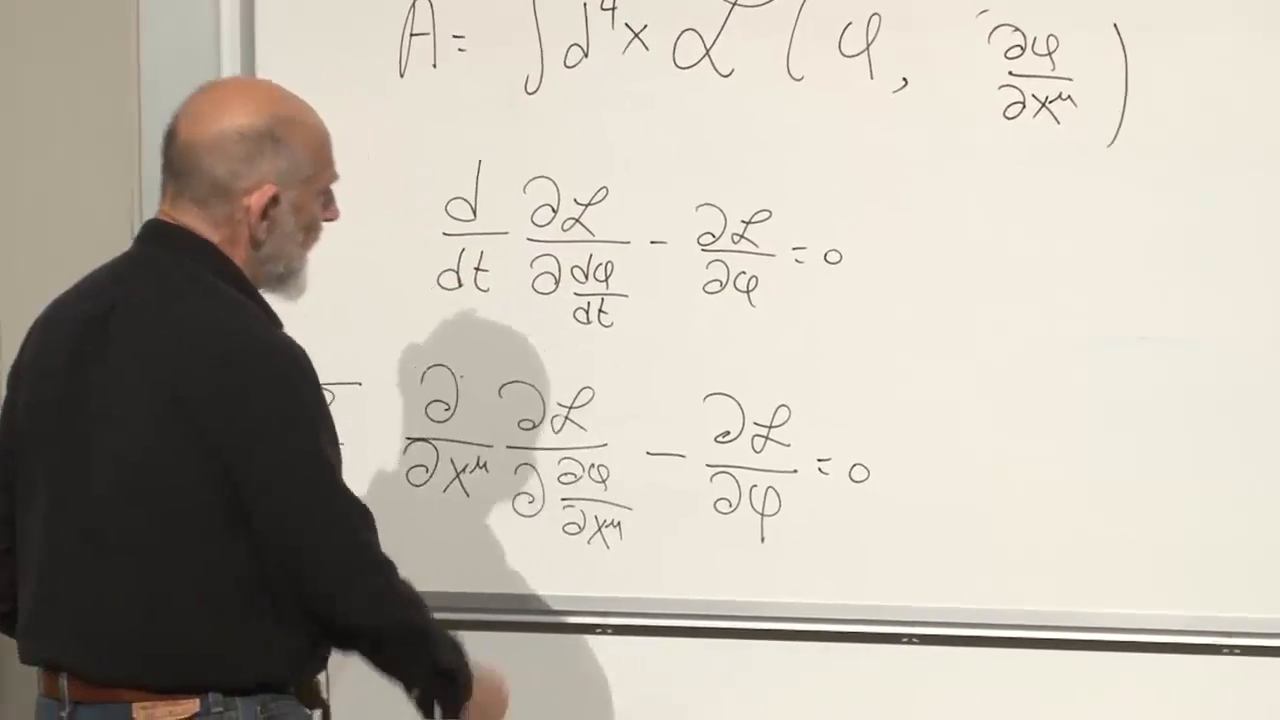
\includegraphics[width=0.90\textwidth]{lecture_04_figure_05.png}
\caption{La densidad de acción expresada como una función local de \(\phi\) y sus derivadas espaciotemporales.}
\lectureframe{00:32:51}
\end{figure}

\begin{classroomqa}
\audiencequestion{¿Puede depender también la densidad lagrangiana de las propias coordenadas \(x,y,z\)?}
\lecturerresponse{Puede, igual que un lagrangiano de partículas puede depender explícitamente de \(t\). En un sistema cerrado e invariante bajo traslaciones, normalmente no depende de ellas, pero la dependencia explícita de las coordenadas no invalida el formalismo. \lecturetimestamp{00:30:29}}
\end{classroomqa}

\begin{classroomqa}
\audiencequestion{¿La construcción hasta aquí es específica de un campo escalar o es general?}
\lecturerresponse{Hasta aquí, el patrón variacional es general. Escribir una sola componente sugiere un campo escalar. Un campo vectorial o una colección de campos tendría etiquetas de componente adicionales, y se variaría cada componente. \lecturetimestamp{00:31:00}}
\end{classroomqa}

\subsection{La representación en una retícula}

En una retícula espaciotemporal fina, las derivadas se convierten en diferencias finitas entre valores del campo en puntos vecinos. La acción es entonces una función ordinaria de muchas variables. Una cuadrícula con 10 puntos en una dirección y 8 en otra ya da 80 variables de campo. Refinar la cuadrícula aumenta su número, pero la regla de minimización sigue siendo elemental: derivar la acción con respecto al valor del campo en cada punto interior e igualar el resultado a cero.

\begin{figure}[htbp]
\centering
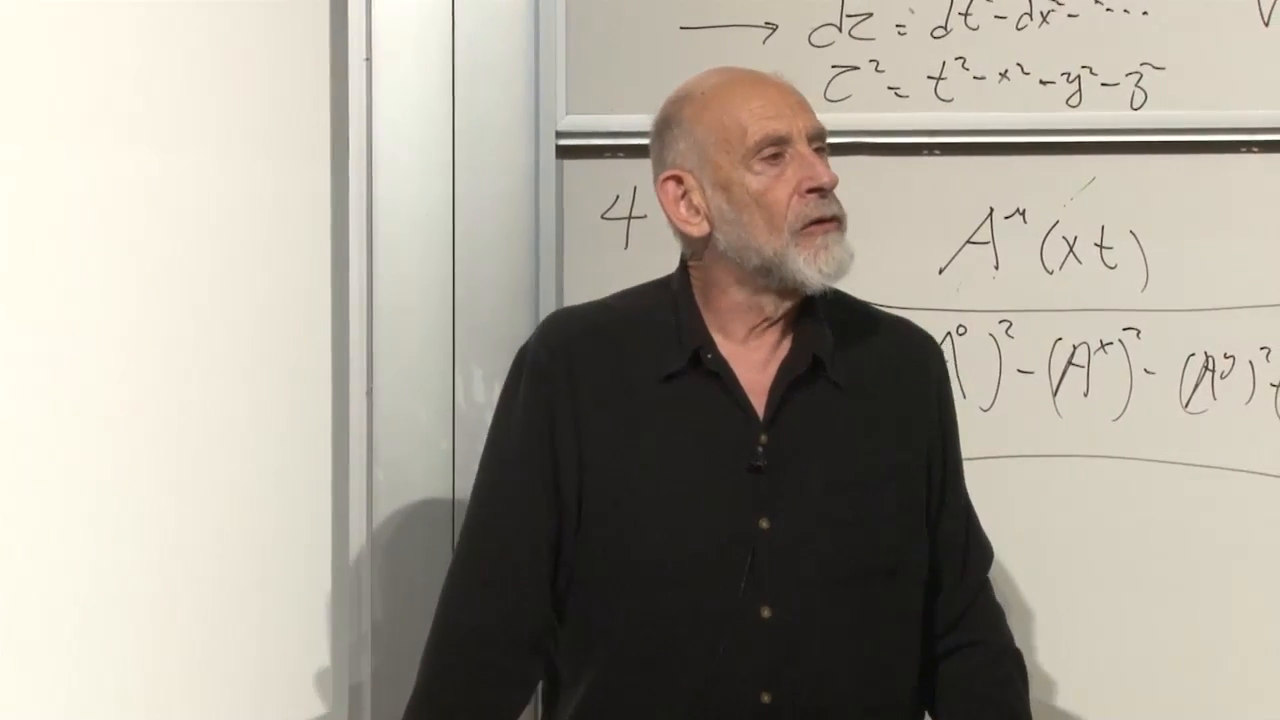
\includegraphics[width=0.90\textwidth]{lecture_04_figure_06.png}
\caption{La región del espacio-tiempo dividida en celdas, lo que convierte la acción en una función ordinaria de muchas variables antes de tomar el límite continuo.}
\lectureframe{00:34:05}
\end{figure}

Al tomar el límite continuo se obtiene la ecuación de Euler--Lagrange del campo:
\begin{equation}
\boxed{
\partial_\mu
\left[
\frac{\partial\mathcal{L}}
{\partial(\partial_\mu\phi)}
\right]
-
\frac{\partial\mathcal{L}}{\partial\phi}
=0
}.
\label{eq:sr4-field-el}
\end{equation}
Se suma repetidamente \(\mu\) sobre todas las direcciones del espacio-tiempo. Escrita sin la abreviatura de sumación, la misma ecuación es
\begin{align}
&
\frac{\partial}{\partial t}
\left(\frac{\partial\mathcal{L}}{\partial\phi_t}\right)
+
\frac{\partial}{\partial x}
\left(\frac{\partial\mathcal{L}}{\partial\phi_x}\right)
+
\frac{\partial}{\partial y}
\left(\frac{\partial\mathcal{L}}{\partial\phi_y}\right)
\nonumber\\
&\hspace{3em}
+
\frac{\partial}{\partial z}
\left(\frac{\partial\mathcal{L}}{\partial\phi_z}\right)
-
\frac{\partial\mathcal{L}}{\partial\phi}
=0.
\label{eq:sr4-field-el-expanded}
\end{align}
El primer término es el término conocido de la mecánica de partículas. La teoría de campos añade un término análogo por cada dirección espacial. El último término, \(-\partial\mathcal{L}/\partial\phi\), no cambia.

\begin{figure}[htbp]
\centering
\includegraphics[width=0.90\textwidth]{lecture_04_figure_07.png}
\caption{La ecuación de Euler--Lagrange unidimensional y su generalización espaciotemporal, escritas una debajo de la otra.}
\lectureframe{00:38:44}
\end{figure}

Este tema también se denomina mecánica del continuo. Según cuáles sean los grados de libertad, las mismas matemáticas pueden describir el flujo de un fluido, la deformación elástica u otro medio continuo.

\begin{classroomqa}
\audiencequestion{¿Funcionarían las mismas ecuaciones en un mundo con espacio, pero sin tiempo?}
\lecturerresponse{Sí, como problema variacional puramente espacial. Físicamente, así se busca una solución estática: se supone que el campo no depende del tiempo, se descartan todas las derivadas temporales y se resuelven las ecuaciones espaciales restantes. Una configuración eléctrica o magnética independiente del tiempo es un ejemplo. \lecturetimestamp{00:40:05}}
\end{classroomqa}

\section{Cómo conjeturar la dinámica escalar más sencilla}

\subsection{Por qué los signos no pueden ser todos iguales}

Volvamos al término cinético de la partícula \(\tfrac12\dot\phi^2\), fijemos en 1 su coeficiente global, que no es relevante, e intentemos generalizarlo. Una primera conjetura podría ser
\begin{equation}
\mathcal{L}_{+}
=
\frac12
\left[
\phi_t^2+\phi_x^2+\phi_y^2+\phi_z^2
\right].
\label{eq:sr4-all-plus}
\end{equation}
Este es un desvío útil, aunque equivocado. Trata el tiempo y el espacio con signos idénticos. La ecuación resultante no tendría la estructura hiperbólica de la propagación de ondas. La combinación relativista correcta asigna un signo al tiempo y el opuesto al espacio.

\begin{classroomqa}
\audiencequestion{¿La expresión con todos los signos positivos es incorrecta porque el lagrangiano debería ser relativistamente invariante?}
\lecturerresponse{Esa es la respuesta más profunda y es correcta. La clase llega primero a los signos por una vía más elemental: las ondas distinguen la evolución temporal de la variación espacial, por lo que el tiempo no puede entrar exactamente igual que otra coordenada espacial. La invariancia de Lorentz pronto convertirá esa intuición en una regla precisa. \lecturetimestamp{00:43:19}}
\end{classroomqa}

Al reintroducir una velocidad característica \(c\), la densidad lagrangiana escalar sencilla es
\begin{equation}
\boxed{
\mathcal{L}
=
\frac12
\left[
\frac{1}{c^2}\phi_t^2
-\phi_x^2-\phi_y^2-\phi_z^2
\right]
-V(\phi)
}.
\label{eq:sr4-scalar-lagrangian}
\end{equation}
En un campo relativista, \(c\) es la velocidad de la luz. En un modelo continuo, podría ser, en cambio, la velocidad del sonido, la de una onda elástica u otra velocidad característica de propagación.

El factor global \(1/2\) es convencional, igual que en \(\tfrac12m\dot\phi^2\). Multiplicar una acción entera por una constante no nula no cambia sus trayectorias estacionarias; esta convención fija cómo se nombran y normalizan los parámetros de las ecuaciones. Una vez elegida esa normalización, hay que usarla de manera coherente.

\begin{classroomqa}
\audiencequestion{¿Se pueden considerar los términos de gradiente espacial parte de la energía potencial?}
\lecturerresponse{Sí. En la organización de energía cinética menos energía potencial, la parte cinética contiene derivadas temporales. Los términos sin derivadas temporales, incluidos los gradientes espaciales y \(V(\phi)\), pertenecen al lado de la energía potencial. En última instancia, el motivo de su signo relativo en una teoría relativista es la métrica lorentziana. \lecturetimestamp{00:45:37}}
\end{classroomqa}

\subsection{La ecuación de onda}

Apliquemos \eqref{eq:sr4-field-el}. Los términos con derivadas son
\begin{equation}
\frac{\partial\mathcal{L}}{\partial\phi_t}
=\frac{1}{c^2}\phi_t,
\qquad
\frac{\partial\mathcal{L}}{\partial\phi_i}
=-\phi_i,
\end{equation}
mientras que
\begin{equation}
\frac{\partial\mathcal{L}}{\partial\phi}
=-\frac{dV}{d\phi}.
\end{equation}
Por tanto,
\begin{equation}
\begin{aligned}
&\boxed{
\frac{1}{c^2}\frac{\partial^2\phi}{\partial t^2}
-\nabla^2\phi
+\frac{dV}{d\phi}
=0
},\\[0.5em]
\nabla^2
&=
\frac{\partial^2}{\partial x^2}
+\frac{\partial^2}{\partial y^2}\\
&\quad
+\frac{\partial^2}{\partial z^2}.
\end{aligned}
\label{eq:sr4-general-scalar-eom}
\end{equation}

Si \(V=0\), esto se reduce a
\begin{equation}
\boxed{
\frac{1}{c^2}\phi_{tt}-\nabla^2\phi=0
},
\label{eq:sr4-wave-equation}
\end{equation}
la ecuación de onda. La clase reconoce la ecuación, pero deja para más adelante su resolución. Sus soluciones propagan perturbaciones a velocidad \(c\).

\begin{figure}[htbp]
\centering
\includegraphics[width=0.90\textwidth]{lecture_04_figure_08.png}
\caption{La forma unidimensional \(c^{-2}\phi_{tt}-\phi_{xx}=0\), reconocida como la ecuación de onda.}
\lectureframe{00:50:30}
\end{figure}

\subsection{Un campo de osciladores armónicos acoplados}

Elijamos ahora un potencial cuadrático:
\begin{equation}
V(\phi)=\frac12\mu^2\phi^2,
\qquad
\frac{dV}{d\phi}=\mu^2\phi.
\label{eq:sr4-quadratic-potential}
\end{equation}
Si \(\phi\) fuera la posición de una partícula, este sería el potencial de un oscilador armónico con constante elástica \(\mu^2\). Para el campo,
\begin{equation}
\boxed{
\frac{1}{c^2}\phi_{tt}-\nabla^2\phi+\mu^2\phi=0
}.
\label{eq:sr4-klein-gordon}
\end{equation}
Sin la derivada espacial, esto no es más que aceleración más una constante por el desplazamiento, igual a cero. El gradiente acopla puntos vecinos y convierte el oscilador en un continuo capaz de soportar ondas. En teoría relativista de campos, \eqref{eq:sr4-klein-gordon} se denomina ecuación de Klein--Gordon masiva; clásicamente, \(\mu\) es la escala de longitud inversa que modifica la propagación de las ondas.

\begin{figure}[htbp]
\centering
\includegraphics[width=0.90\textwidth]{lecture_04_figure_09.png}
\caption{El potencial cuadrático y la ecuación de onda resultante con el término restaurador \(\mu^2\phi\).}
\lectureframe{00:52:38}
\end{figure}

\begin{classroomqa}
\audiencequestion{¿Por qué desaparece de la ecuación de movimiento el factor \(1/2\) de \(V=\tfrac12\mu^2\phi^2\)?}
\lecturerresponse{Derivar \(\phi^2\) aporta un factor de 2. El factor convencional \(1/2\) se introduce precisamente para que \(dV/d\phi=\mu^2\phi\), igual que \(V(x)=\tfrac12kx^2\) da la fuerza restauradora \(-kx\). \lecturetimestamp{00:53:17}}
\end{classroomqa}

La ecuación es lineal: \(\phi\) y cada una de sus derivadas aparecen solo a la primera potencia. Términos como \(\phi^2\) o \(\phi\,\partial_\mu\phi\) en la ecuación de movimiento harían que la dinámica fuera no lineal.

\section{Escalares de Lorentz y cuadrivectores}

\subsection{La acción debe ser independiente del sistema de referencia}

El formalismo variacional por sí solo define muchas teorías de campos posibles. La relatividad impone el requisito adicional de que la acción tenga el mismo valor y la misma forma en todos los sistemas de referencia inerciales. Para la partícula libre, esto se conseguía integrando el tiempo propio invariante \(d\tau\) a lo largo de la línea de universo. Para un campo, la acción se integra sobre el espacio-tiempo, de modo que sus elementos locales deben transformarse como corresponde.

La medida del espacio-tiempo es invariante bajo una transformación de Lorentz propia: \(d^4x'=d^4x\). Por tanto, basta exigir que la densidad lagrangiana sea un escalar de Lorentz:
\begin{equation}
\mathcal{L}'(x')=\mathcal{L}(x).
\label{eq:sr4-lagrangian-scalar}
\end{equation}

\subsection{Campos escalares}

Un campo escalar obedece la ley
\begin{equation}
\boxed{\phi'(x')=\phi(x)}.
\label{eq:sr4-scalar-transform}
\end{equation}
Las coordenadas \(x\) y \(x'\) designan el mismo suceso en dos sistemas de referencia. Las expresiones funcionales que usan los observadores pueden parecer distintas, pero el número asociado a ese suceso físico es el mismo.

\begin{figure}[htbp]
\centering
\includegraphics[width=0.90\textwidth]{lecture_04_figure_10.png}
\caption{La ley de transformación que define un campo escalar: \(\phi(x)=\phi'(x')\).}
\lectureframe{00:59:33}
\end{figure}

La temperatura ofreció una intuición inicial, aunque un termómetro en movimiento dentro de un medio material no constituye un ejemplo relativista perfecto. Lo que importa es la definición \eqref{eq:sr4-scalar-transform}, no la analogía del termómetro.

\subsection{Cuadrivectores}

En unidades \(c=1\), un impulso de velocidad \(v\) a lo largo del eje \(x\) actúa como
\begin{equation}
\begin{aligned}
t'&=\gamma(t-vx),\\
x'&=\gamma(x-vt),\\
y'&=y,\\
z'&=z,\\
\gamma&=\frac{1}{\sqrt{1-v^2}}.
\end{aligned}
\label{eq:sr4-x-boost}
\end{equation}

\begin{figure}[htbp]
\centering
\includegraphics[width=0.90\textwidth]{lecture_04_figure_11.png}
\caption{La transformación de Lorentz correspondiente a un impulso a lo largo del eje \(x\), en unidades \(c=1\).}
\lectureframe{01:02:26}
\end{figure}

Cuatro magnitudes cualesquiera que se mezclen del mismo modo bajo impulsos forman un cuadrivector. Entre los ejemplos ya vistos están \(x^\mu\), \(dx^\mu\) y la cuadrivelocidad \(u^\mu=dx^\mu/d\tau\). El producto de un cuadrivector por un escalar es otro cuadrivector. Un fluido relativista en movimiento ofrece un ejemplo de campo vectorial: su cuadrivelocidad \(u^\mu(x)\) puede variar de un suceso a otro.

Para el mismo impulso que en \eqref{eq:sr4-x-boost}, un cuadrivector genérico obedece
\begin{equation}
\begin{aligned}
A'^0&=\gamma(A^0-vA^x),\\
A'^x&=\gamma(A^x-vA^0),\\
A'^y&=A^y,\\
A'^z&=A^z.
\end{aligned}
\label{eq:sr4-vector-boost}
\end{equation}

Para un cuadrivector genérico \(A^\mu=(A^0,A^x,A^y,A^z)\), la norma lorentziana
\begin{equation}
\boxed{
A_\mu A^\mu
=(A^0)^2-(A^x)^2-(A^y)^2-(A^z)^2
}
\label{eq:sr4-vector-norm}
\end{equation}
es un escalar. Es invariante por el mismo motivo algebraico por el que es invariante \begin{equation}
d\tau^2=dt^2-dx^2-dy^2-dz^2
\end{equation}. En la clase se agotan brevemente las letras disponibles para un vector genérico antes de aceptar \(A\), gracias a la sugerencia de usar \(A\) por la flecha.

\begin{figure}[htbp]
\centering
\includegraphics[width=0.90\textwidth]{lecture_04_figure_12.png}
\caption{Un campo cuadrivectorial genérico y la diferencia lorentziana de cuadrados con la que se forma su norma invariante.}
\lectureframe{01:09:06}
\end{figure}

\subsection{La derivada de un escalar}

Al derivar un escalar con respecto a las 4 coordenadas del espacio-tiempo se obtienen las 4 componentes
\begin{equation}
\partial_\mu\phi
=
\left(
\frac{\partial\phi}{\partial t},
\frac{\partial\phi}{\partial x},
\frac{\partial\phi}{\partial y},
\frac{\partial\phi}{\partial z}
\right)
\qquad(c=1).
\end{equation}
En sentido estricto, \(\partial_\mu\phi\) es un covector; la métrica de Minkowski eleva su índice para obtener \(\partial^\mu\phi\). Esta distinción no afecta al argumento por componentes de aquí, pero permite definir sin ambigüedad la contracción:
\begin{equation}
\boxed{
\partial_\mu\phi\,\partial^\mu\phi
=
\frac{1}{c^2}\phi_t^2
-\phi_x^2-\phi_y^2-\phi_z^2
}.
\label{eq:sr4-derivative-scalar}
\end{equation}

\begin{figure}[htbp]
\centering
\includegraphics[width=0.90\textwidth]{lecture_04_figure_13.png}
\caption{La diferencia invariante de cuadrados formada a partir de las primeras derivadas de un campo escalar.}
\lectureframe{01:13:55}
\end{figure}

\begin{classroomqa}
\audiencequestion{¿Es laplaciano esta combinación de derivadas?}
\lecturerresponse{No. El invariante mostrado es cuadrático en las primeras derivadas. El laplaciano contiene segundas derivadas espaciales. Las segundas derivadas aparecen solo al variar la acción, en la ecuación de onda. \lecturetimestamp{01:13:22}}
\end{classroomqa}

Ahora queda explicado, en vez de conjeturado, el patrón de signos de \eqref{eq:sr4-scalar-lagrangian}. La combinación de los términos cinético y de gradiente es el escalar de Lorentz \(\partial_\mu\phi\,\partial^\mu\phi\). Así, la teoría cuadrática más sencilla es
\begin{equation}
\mathcal{L}
=
\frac12\partial_\mu\phi\,\partial^\mu\phi
-\frac12\mu^2\phi^2.
\label{eq:sr4-covariant-lagrangian}
\end{equation}

\begin{figure}[htbp]
\centering
\includegraphics[width=0.90\textwidth]{lecture_04_figure_14.png}
\caption{La densidad lagrangiana cuadrática escalar completa y su ecuación lineal de campo en la pizarra.}
\lectureframe{01:19:12}
\end{figure}

\section{¿Cuánta libertad hay?}

Una vez conocida la regla para construir escalares, son posibles muchos lagrangianos. El campo \(\phi\) es escalar, así que cualquier función ordinaria \(F(\phi)\) también es escalar: \(\phi^2\), \(\phi^3\), \(\cosh\phi\), etc. También se permiten parámetros numéricos. Se puede introducir un símbolo como \(\mu\) como coeficiente constante; las únicas cuestiones pendientes son sus dimensiones y su interpretación física.

\begin{classroomqa}
\audiencequestion{¿Se puede incluir una masa en el lagrangiano?}
\lecturerresponse{Sin duda se puede incluir un parámetro constante. En esta etapa conviene preguntarse de qué objeto es la masa, porque \(\mu\) no es más que un número en la teoría clásica de campos hasta que se identifica su significado físico. En la teoría escalar relativista cuadrática, fija la masa o la escala de longitud inversa. \lecturetimestamp{01:14:16}}
\end{classroomqa}

Se pueden multiplicar escalares:
\begin{equation}
F(\phi)\,\partial_\mu\phi\,\partial^\mu\phi
\end{equation}
es invariante de Lorentz. También se puede elevar al cuadrado el propio escalar de las derivadas, lo que produce potencias superiores de las primeras derivadas. Asimismo, se pueden considerar derivadas de orden superior, aunque la clase se limita a los campos y sus primeras derivadas, el marco estándar que da lugar a ecuaciones de movimiento de segundo orden. Las teorías con derivadas de orden superior requieren más cuidado porque, en general, introducen datos dinámicos adicionales y posibles inestabilidades.

\begin{classroomqa}
\audiencequestion{¿La construcción de la diferencia de cuadrados es realmente la métrica del espacio-tiempo?}
\lecturerresponse{Sí. Con la signatura elegida, la métrica es \(dt^2-dx^2-dy^2-dz^2\). La clase todavía no ha destacado la palabra métrica, pero esta es exactamente la geometría del espacio-tiempo que será fundamental en la relatividad general. \lecturetimestamp{01:19:39}}
\end{classroomqa}

\begin{classroomqa}
\audiencequestion{¿Hay objetos más generales que los cuadrivectores, con componentes como \(xy\) o \(tx\)?}
\lecturerresponse{Sí. Son tensores. Un escalar no tiene índice espaciotemporal, un vector tiene uno y un tensor de rango 2 tiene componentes como \(T^{xx}\), \(T^{xy}\) y \(T^{tx}\). La mayor parte de la discusión actual sobre campos escalares los evita; en relatividad general se vuelven inevitables. \lecturetimestamp{01:20:49}}
\end{classroomqa}

\begin{classroomqa}
\audiencequestion{¿Por qué se consideran solo impulsos que mezclan \(t\) con \(x\)? ¿Podría un impulso apuntar en otra dirección y mezclar los ejes espaciales de otro modo?}
\lecturerresponse{Por supuesto. Un impulso a lo largo de \(y\) mezcla \(t\) con \(y\) y deja \(x,z\) sin cambios. Una transformación de Lorentz general se puede construir combinando rotaciones espaciales con un impulso a lo largo del eje elegido. Por tanto, basta con establecer la invariancia bajo rotaciones y bajo un impulso estándar a lo largo de un eje. \lecturetimestamp{01:22:06}}
\end{classroomqa}

\begin{classroomqa}
\audiencequestion{Con tantas combinaciones escalares posibles, ¿describen todos los lagrangianos resultantes una física significativa?}
\lecturerresponse{A nivel clásico, la libertad es inmensa, sujeta a requisitos adicionales como signos razonables, localidad y un problema de evolución bien planteado. Muchas menos elecciones arbitrarias definen teorías cuánticas fundamentales bien comportadas. La teoría cuántica de campos efectiva moderna admite muchas otras interacciones por debajo de una escala de corte, pero entonces hay que especificar su intervalo de validez. \lecturetimestamp{01:27:57}}
\end{classroomqa}

\begin{classroomqa}
\audiencequestion{¿Tiene que ser continuo un campo?}
\lecturerresponse{En las teorías suaves que estamos considerando, sí. Un salto produce derivadas singulares y, con un término cuadrático de gradiente, normalmente acción y energía infinitas. Las configuraciones más singulares solo pueden tratarse incorporando estructura matemática adicional; no son los campos ordinarios de energía finita que estamos desarrollando aquí. \lecturetimestamp{01:29:29}}
\end{classroomqa}

\section{Una partícula acoplada a un campo escalar}

\subsection{La partícula libre, revisitada}

La parte final de la clase combina partículas y campos a nivel clásico. Todavía no se trata del enunciado cuántico según el cual las partículas son excitaciones de campos. Supongamos, en cambio, que alguien ya ha resuelto el campo escalar de fondo \(\phi(x,t)\) y preguntémonos cómo se mueve una partícula a través de él.

Para una partícula relativista libre,
\begin{equation}
A_{\rm free}=-m\int d\tau.
\label{eq:sr4-free-particle-action}
\end{equation}
En una dimensión espacial y con \(c=1\),
\begin{equation}
d\tau=dt\sqrt{1-\dot x^2},
\qquad
L_{\rm free}=-m\sqrt{1-\dot x^2}.
\label{eq:sr4-free-particle-l}
\end{equation}
Se elige el signo menos para que la expansión a velocidades bajas dé el término cinético newtoniano positivo habitual:
\begin{equation}
L_{\rm free}
\approx -m+\frac12m\dot x^2+\cdots.
\end{equation}

\begin{figure}[htbp]
\centering
\includegraphics[width=0.90\textwidth]{lecture_04_figure_15.png}
\caption{La acción invariante de la partícula libre, reescrita como lagrangiano en función del tiempo coordenado.}
\lectureframe{01:34:31}
\end{figure}

\subsection{El acoplamiento escalar más sencillo}

Tanto \(d\tau\) como \(\phi\) son escalares. Por tanto, el acoplamiento lineal más sencillo es
\begin{equation}
\boxed{
A
=
\int d\tau\,[-m+\phi(x,t)]
}.
\label{eq:sr4-coupled-action}
\end{equation}
Esta elección no es única. Se podría sustituir \(\phi\) por cualquier función
\(F(\phi)\). El término lineal basta para ilustrar la idea física.

\begin{figure}[htbp]
\centering
\includegraphics[width=0.90\textwidth]{lecture_04_figure_16.png}
\caption{La acción libre complementada con el acoplamiento escalar invariante de Lorentz más sencillo.}
\lectureframe{01:37:21}
\end{figure}

\begin{classroomqa}
\audiencequestion{¿Tiene que permanecer \(\phi\) dentro de la integral?}
\lecturerresponse{Sí. El campo se evalúa sobre la línea de universo de la partícula, \(\phi(x(t),t)\), y por lo general cambia de un punto de la trayectoria a otro. Aunque el fondo no dependa explícitamente del tiempo, \(\phi=\phi(x)\), el campo sigue cambiando con el tiempo cuando la partícula se mueve por el espacio. Solo se podría sacar de la integral un campo constante a lo largo del recorrido. \lecturetimestamp{01:37:47}}
\end{classroomqa}

\begin{classroomqa}
\audiencequestion{¿La \(x\) de \(\phi(x,t)\) representa la posición de la partícula?}
\lecturerresponse{Sí. Es \(x=x(t)\), la posición de la partícula en el instante \(t\). La acción evalúa el campo espaciotemporal prescrito a lo largo de esa trayectoria. \lecturetimestamp{01:38:08}}
\end{classroomqa}

Para el movimiento en una dimensión, \eqref{eq:sr4-coupled-action} da
\begin{equation}
L
=
-(m-\phi(x,t))\sqrt{1-\dot x^2}.
\label{eq:sr4-coupled-lagrangian}
\end{equation}
El fondo escalar aparece exactamente en el lugar que ocupa la masa en reposo:
\begin{equation}
m_{\rm eff}(x,t)=m-\phi(x,t).
\label{eq:sr4-effective-mass}
\end{equation}
Si \(\phi\) se estabiliza en un valor no nulo casi constante, la partícula se comporta como si su masa hubiera cambiado. Este es solo un modelo clásico de juguete, no el mecanismo de Higgs completo, pero capta el rasgo característico de la idea del Higgs que se quería presentar: un fondo escalar puede intervenir en la dinámica de una partícula como término de masa.

\subsection{La ecuación de movimiento de la partícula}

El momento canónico es
\begin{equation}
p
=
\frac{\partial L}{\partial\dot x}
=
(m-\phi)
\frac{\dot x}{\sqrt{1-\dot x^2}}.
\label{eq:sr4-coupled-momentum}
\end{equation}

\begin{figure}[htbp]
\centering
\includegraphics[width=0.90\textwidth]{lecture_04_figure_17.png}
\caption{El fondo escalar sustituye \(m\) por \(m-\phi(x,t)\) en el momento canónico relativista.}
\lectureframe{01:43:38}
\end{figure}

La derivada del lagrangiano respecto de la posición es
\begin{equation}
\frac{\partial L}{\partial x}
=
\frac{\partial\phi}{\partial x}
\sqrt{1-\dot x^2}.
\end{equation}
Con el signo fijado por la acción
\eqref{eq:sr4-coupled-action}, la ecuación de Euler--Lagrange es, por tanto,
\begin{equation}
\boxed{
\frac{d}{dt}
\left[
(m-\phi)
\frac{\dot x}{\sqrt{1-\dot x^2}}
\right]
=
\frac{\partial\phi}{\partial x}
\sqrt{1-\dot x^2}
}.
\label{eq:sr4-coupled-eom}
\end{equation}

\begin{figure}[htbp]
\centering
\includegraphics[width=0.90\textwidth]{lecture_04_figure_18.png}
\caption{La ecuación de movimiento acoplada se construye a partir del momento y de la derivada espacial del campo de fondo; la acción fija el signo final en \eqref{eq:sr4-coupled-eom}.}
\lectureframe{01:45:24}
\end{figure}

\begin{classroomqa}
\audiencequestion{¿Por qué \(\partial\phi/\partial x\) conserva el factor \(\sqrt{1-\dot x^2}\)?}
\lecturerresponse{Porque solo se deriva el factor \(\phi(x,t)\) con respecto a \(x\). En el lagrangiano, la raíz cuadrada lo multiplica y no depende de la posición cuando \(\dot x\) se mantiene fija al calcular la derivada parcial; por eso la raíz cuadrada permanece. \lecturetimestamp{01:45:50}}
\end{classroomqa}

Al desarrollar la derivada total respecto del tiempo se obtiene
\begin{align}
&(m-\phi)
\frac{d}{dt}
\left(
\frac{\dot x}{\sqrt{1-\dot x^2}}
\right)
-
\dot\phi\,
\frac{\dot x}{\sqrt{1-\dot x^2}}
\nonumber\\
&\hspace{10em}
=
\frac{\partial\phi}{\partial x}
\sqrt{1-\dot x^2}.
\label{eq:sr4-coupled-expanded}
\end{align}
Si el fondo es estático, \(\phi=\phi(x)\), su derivada a lo largo de la línea de universo en movimiento no es cero. La regla de la cadena da
\begin{equation}
\boxed{
\dot\phi
=
\frac{d}{dt}\phi(x(t))
=
\frac{\partial\phi}{\partial x}\dot x
}.
\label{eq:sr4-chain-rule}
\end{equation}

\begin{classroomqa}
\audiencequestion{Si \(\phi\) no depende explícitamente del tiempo, ¿por qué \(\dot\phi\) no es cero?}
\lecturerresponse{Porque la partícula cambia de posición. El campo se evalúa en \(x(t)\), así que su derivada total es \(\dot\phi=\phi_x\dot x\). Que el campo sea estático significa \(\partial\phi/\partial t=0\), no que toda partícula en movimiento perciba un valor constante del campo. \lecturetimestamp{01:48:10}}
\end{classroomqa}

\begin{figure}[htbp]
\centering
\includegraphics[width=0.90\textwidth]{lecture_04_figure_19.png}
\caption{Desarrollo final de la ecuación de movimiento acoplada tras aplicar la regla de la cadena a lo largo de la línea de universo.}
\lectureframe{01:49:11}
\end{figure}

La expresión exacta no es especialmente elegante, y la clase no pretende lo contrario. Sin embargo, su límite de velocidades bajas resulta familiar. Puesto que
\(\sqrt{1-\dot x^2}\approx1\), la ecuación de orden principal es
\begin{equation}
\frac{d}{dt}\bigl[(m-\phi)\dot x\bigr]
\approx
\frac{\partial\phi}{\partial x}.
\end{equation}
Si además se trata perturbativamente la variación de la masa efectiva, se obtiene
\begin{equation}
(m-\phi)\ddot x
\approx
\frac{\partial\phi}{\partial x}.
\label{eq:sr4-nonrel-force}
\end{equation}
En efecto, el lagrangiano a bajas velocidades es
\begin{equation}
L
\approx
-m+\phi+\frac12(m-\phi)\dot x^2,
\end{equation}
Así que, en el orden principal, la energía potencial es \(U=-\phi\) y la fuerza es
\(-dU/dx=\partial_x\phi\). Restablecer los factores de \(c\) y recuperar este patrón newtoniano es el ejercicio con el que termina la clase.

Ya está completo el recorrido que va de las partículas a los campos. La historia de una partícula \(\phi(t)\) proporcionó el prototipo en \(0+1\) dimensiones; la historia de un campo \(\phi(x)\) convirtió la acción en una integral espaciotemporal; la ecuación de Euler--Lagrange del campo produjo la dinámica de ondas; los escalares de Lorentz determinaron la estructura de signos relativista; y el mismo lenguaje invariante permitió que un fondo escalar influyera a su vez en una partícula.
